The following Sections describe the methods used in the course of this thesis.

\subsection{Visual Features Variational Autoencoders}\label{subsec:visual-features-variational-autoencoders}
Different questions were asked investigate whether \acp{VAE} are a biologically plausible model of the Visual Cortex.

One essential prerequisite is the emergence of Gabor wavelets (\textbf{Ref}).
As discussed in Section~\ref{subsec:visual_features_in_neural_networks}, Gabor wavelets do emerge in deep convolutional networks, trained on image classification~\citep{krizhevsky2012imagenet} (\textbf{Ref: at least one more paper }), specifically on the ImageNet dataset (\textbf{ref}).\par
The following approaches were taken to see if Gabor wavelets do naturally emerge in \acp{VAE} (\textbf{explain ``naturally"}).\par
First, the convolutional kernels in a \ac{VAE} that was sucessfully trained on the CelebA (\textbf{ref}) dataset in terms of image reconstruction were examined in terms of emergence of Gabor wavelets (\textbf{explain network architecture}).
Subsequently, the size of the convolutional kernels in the first layer was increased to size 11x11 \footnote{This is the same kernel size of the first layers used in~\citet{krizhevsky2012imagenet}.} as they were too small to successfully represent any Gabor wavelets~\citep{han2019variational}.
Since still no Gabor wavelets emerged (see Section~\ref{subsec:results_visual_features_in_variational_autoencoders}), the question was raised whether this was because of the different network architectures of AlexNet and the ``CelebA VAE", or the dataset, or both.

\begin{figure}
    \centering
    \begin{subfigure}{.5\textwidth}
        \centering
        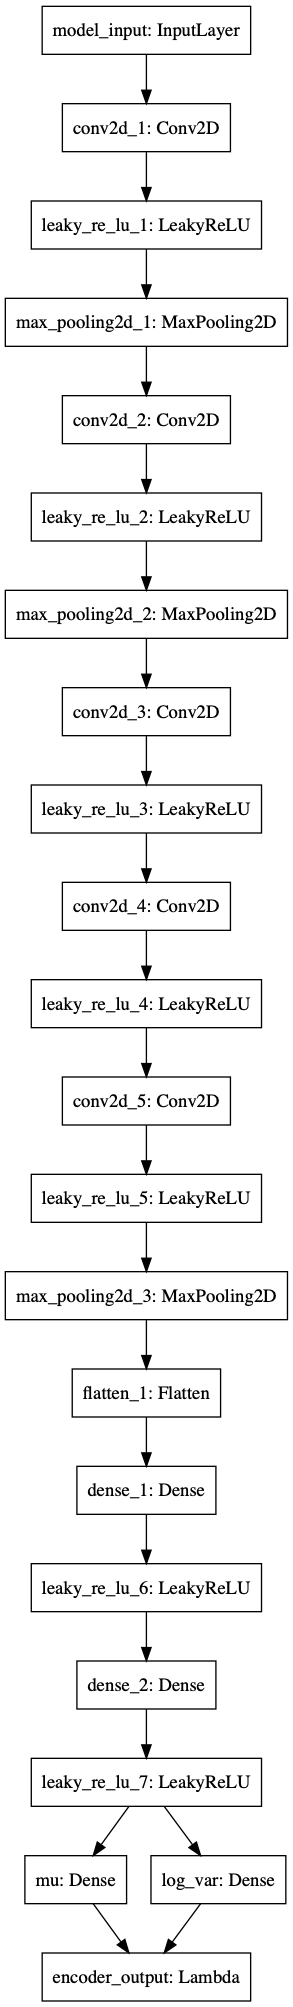
\includegraphics[width=\textwidth,height=.9\textheight,keepaspectratio]{alexnet-vae/encoder.png}
        \caption{Encoder}
    \end{subfigure}%
    \begin{subfigure}{.5\textwidth}
        \centering
        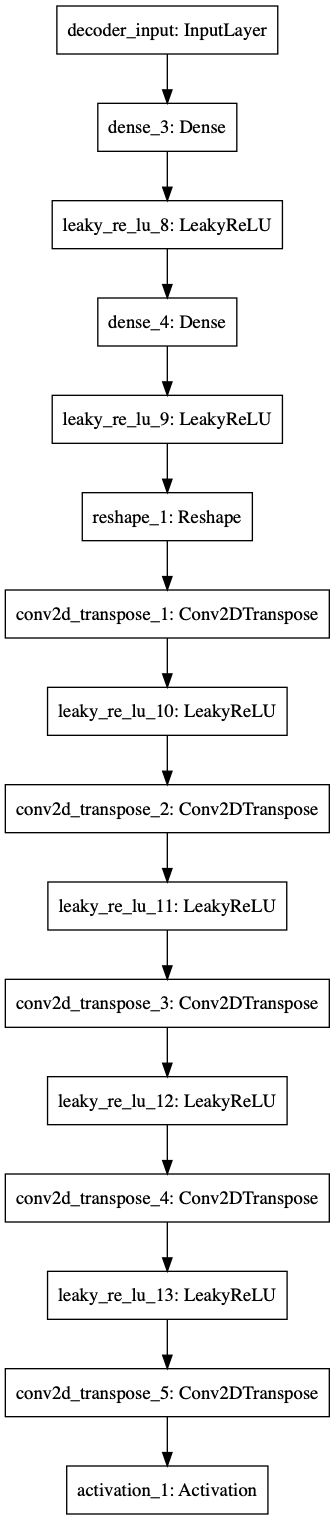
\includegraphics[width=\textwidth,height=.9\textheight,keepaspectratio]{alexnet-vae/decoder.png}
        \caption{Decoder}
    \end{subfigure}
    \caption{AlexNet-VAE Network}
    \label{fig:alexnet-vae-encoder}
\end{figure}

To further localize the so-far cause for the non-existence of Gabor wavelets, an ``AlexNet-like-VAE'' (subsequently called AlexNet-VAE, see Figure~\ref{fig:alexnet-vae-encoder}) was trained on ImageNet.
This \ac{VAE} consists of an encoder part that closely resembles AlexNet.
The output-layer, however, was changed in terms of size and activation function.
First of all, the output size was allowed to be dynamical to allow different embedding sizes, i.e. differently sized multivariate Gaussians.
Also, the activation function was changed from Softmax (\textbf{ref}) to \ac{LeakyReLU} (\textbf{ref}).
Furthermore, all other activations were also changed to \ac{LeakyReLU} due to its advantages over \ac{ReLU} (\textbf{which ones? explain}).
The encoder is was followed by the reparametrization layer and, subsequently, the decoder part which basically consists of the inverse AlexNet structure.\par

\begin{figure}
    \centering
    \begin{center}
        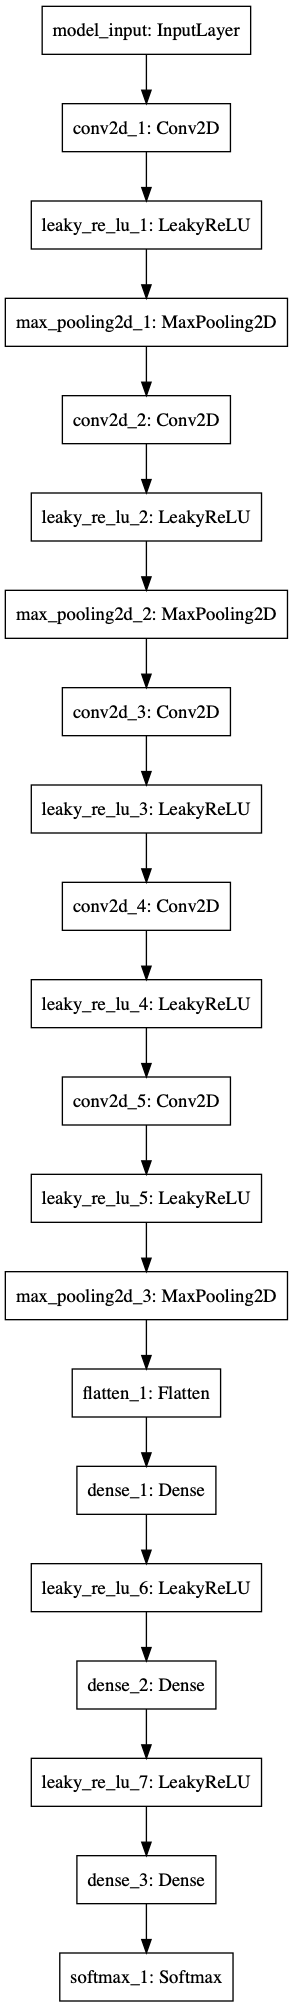
\includegraphics[height=0.9\textheight]{alexnet/model.png}
    \end{center}
    \caption[AlexNet Network]{AlexNet-inspired Image Classification Network}
    \label{fig:alexnet}
\end{figure}

To cross-check the results of the AlexNet-VAE, only the encoder part was trained on ImageNet and image classification, using the Softmax activation in the last layer but keeping the \ac{LeakyReLU} activations in all other layers (see Figure~\ref{fig:alexnet}).

As it turned out that also in the AlexNet-VAE no Gabor wavelets emerged (see Section~\ref{subsec:results_visual_features_in_variational_autoencoders}), the image classification AlexNet-like network was used as an encoder with frozen weights and only the decoder part was trained to see if using a network trained on image classification has certain disadvantages when being used as a decoder in a \ac{VAE} compared to a decoder trained from scratch.